% THIS IS SIGPROC-SP.TEX - VERSION 3.1
% WORKS WITH V3.2SP OF ACM_PROC_ARTICLE-SP.CLS
% APRIL 2009
%
% It is an example file showing how to use the 'acm_proc_article-sp.cls' V3.2SP
% LaTeX2e document class file for Conference Proceedings submissions.
% ----------------------------------------------------------------------------------------------------------------
% This .tex file (and associated .cls V3.2SP) *DOES NOT* produce:
%       1) The Permission Statement
%       2) The Conference (location) Info information
%       3) The Copyright Line with ACM data
%       4) Page numbering
% ---------------------------------------------------------------------------------------------------------------
% It is an example which *does* use the .bib file (from which the .bbl file
% is produced).
% REMEMBER HOWEVER: After having produced the .bbl file,
% and prior to final submission,
% you need to 'insert'  your .bbl file into your source .tex file so as to provide
% ONE 'self-contained' source file.
%
% Questions regarding SIGS should be sent to
% Adrienne Griscti ---> griscti@acm.org
%
% Questions/suggestions regarding the guidelines, .tex and .cls files, etc. to
% Gerald Murray ---> murray@hq.acm.org
%
% For tracking purposes - this is V3.1SP - APRIL 2009

\documentclass{acm_proc_article-sp}
\usepackage{url}
\begin{document}

\title{QueryMed: For Querying Biomedical Data on the Web\titlenote{Interested readers are advised to visit http://code.google.com/p/querymed to learn more about QueryMed.}}


\numberofauthors{2}
\author{
\alignauthor Oshani Seneviratne\\
       \affaddr{Massachusetts Institute of Technology}\\
       \affaddr{Cambridge, MA}\\
       \affaddr{USA}\\
       \email{oshani@csail.mit.edu}
\alignauthor Rachel Sealfon\\
       \affaddr{Massachusetts Institute of Technology}\\
       \affaddr{Cambridge, MA}\\
       \affaddr{USA}\\
       \email{rsealfon@csail.mit.edu}
}


\maketitle
\begin{abstract}

QueryMed is a query builder and result set visualizer for biomedical data that allows users to easily construct and run translational medicine queries across multiple data sources. The system is accessible for users who are unfamiliar with the SPARQL query language 
or the structure of the underlying ontologies. It permits users to retrieve data from an information-rich default set of resources or to draw on their specialized domain knowledge to determine the most appropriate data sources to query.  User input is provided through an intuitive interface, translated into SPARQL~\cite{SPARQL} queries, and executed at the relevant endpoints. The results are presented in an accessible interface that allows query refinement and filtering.  

\end{abstract}

%\category{H.4}{Information Systems Applications}{Miscellaneous}
\keywords{Biomedical Ontologies, SPARQL, Query Federation, Query Building, Semantic Web, User Interfaces} 

\section{Introduction}

The quantity of publicly available data in the biomedical domain has dramatically increased in recent years. With the linked open data movement, the Semantic Web community has been very proactive in converting these rich information datasources to Resource Description Framework (RDF) triplestores~\cite{LinkingData, Yip}.  However, to exploit the abundance of biomedical data on the Semantic Web, there is a need for easy-to-use systems that do not require the end user to have knowledge of the underlying  structure of the data or of the ontologies used in describing the data. These systems should support queries that run across multiple data sources.  There is also a  need for efficient hybrid interfaces that allow browsing data resources as well as performing queries~\cite{Jentzsch}.  

%Her question must be broken up into discrete pieces that can be executed individually at one data source at a time.  Since the physician must search many data sources in order to find an answer to her single question, she requires a system that can automatically run queries over multiple data sources. Also, the physician may not know SPARQL syntax, the location of the SPARQL endpoints (i.e. data sources), or the structure of the ontologies used to describe the data in the endpoints. She is likely to want an intuitive way to query and to display the query results.  Developing intuitive ways to query multiple SPARQL endpoints and to display results is both an important and a challenging problem.  Our system, QueryMed, allows users with no knowledge of the SPARQL query language or the structure of the underlying ontologies to easily run queries across multiple SPARQL endpoints.


\section{Overview}

The QueryMed system is designed to allow users without specialized knowledge of database query languages to browse and query the extensive biomedical data resources available in RDF triplestores. The simple user interface of QueryMed is intuitive for users with no knowledge of SPARQL and allows the user to run queries across multiple biomedical datasources.  Queries can be run against a default list of SPARQL endpoints, or against a set of user-defined endpoints. The system automatically translates the user input into a SPARQL query for each individual endpoint, executes the query, combines the results, and returns them to the user.  The user can choose to refine the query by iteratively modifying the original search terms and by filtering the result set.  The system's advanced query functionality enables the user to construct complex logical SPARQL queries that take advantage of the underlying structure of the data.  A general overview of QueryMed architecture is shown in Figure \ref{fig:arch_details}.

\begin{figure}
\centering
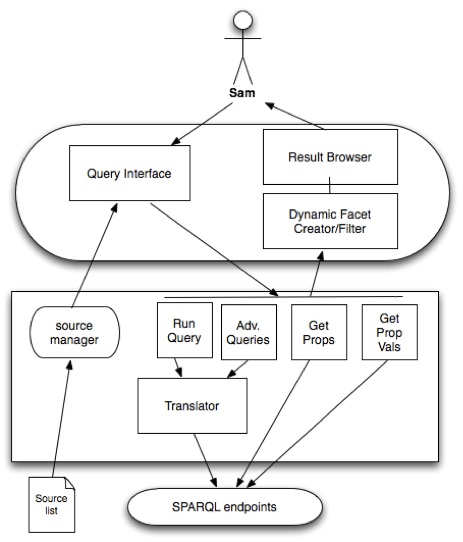
\epsfig{file=images/architecture_detail.jpg, width=3in}
\caption{QueryMed Architecture}
\label{fig:arch_details}
\end{figure}

\subsection{Sample use case}

Imagine a scenario in which a physician, Sam, is interested in locating freely available resources related to coronary artery disease.  Using QueryMed, Sam first runs a basic search by entering ``coronary artery disease" in the search box. He sees a table displaying disease names in the Diseasome database and drugs in DailyMed and Drugbank that relate to coronary artery disease.  He can then filter the results using additional search terms.  For example, he knows that the route of administration of the drug that he is looking for is injection, so he filters the drug query results on the route of administration field using the query term ``injection."  He is now interested in finding relevant clinical trials for his patient.  The clinical trial database (LinkedCT~\cite{LinkedCT}) is not in the default set of endpoints, so he selects the ``Refine Query" option to choose additional endpoints to search.  He sees a list of default endpoints, and selects the ``Add" option to include an additional endpoint.  After entering the name and URL of the LinkedCT endpoint, he is able to search for clinical trials for which his patient may be eligible.  He is also interested in further refining the search, so he uses the advanced search option to search the data available in the Diseasome endpoint for a list of diseases whose class is ``Cardiovascular" or for which the associated gene is ``ABCA1."  Using the QueryMed advanced search interface, the complex SPARQL query corresponding to his question is automatically constructed, and he can view the query results conveniently displayed in a table. A demo illustrating this scenario is available at \url{http://dig.csail.mit.edu/2010/Papers/www-ws-colab-science/videos/querymed-demo.mov}.

\section{Related Work}
\label{related}

A number of existing tools aim to provide a user-friendly interface for browsing Semantic Web data, or to allow users to perform federated queries. The SMART query tool~\cite{Battista} is a Web-based application designed to allow biologists to run queries written in Manchester OWL syntax. GoWeb~\cite{Dietze} allows users to perform a hybrid search, running keyword-based queries and then filtering based on ontological concepts.  BioGateway~\cite{Antezana} provides a Web interface to query a single provided SPARQL endpoint that includes graphs from several biomedical resources.  Another query-building tool, Twinkle~\cite{Dodds}, offers a stand-alone graphical user interface to load and edit SPARQL queries. The DARQ  system \cite{Quilitz} is designed to allow the user to run integrated queries against multiple SPARQL endpoints. But it does not offer a graphical user interface to facilitate use by biomedical domain experts who are not familiar with SPARQL query syntax.

Features of the QueryMed system that distinguish it from similar systems include the ability both to perform keyword queries and to construct more advanced queries taking advantage of the structure of the data, a hybrid interface that enables the user to both query and browse data, and a graphical user interface permitting the dynamic addition of endpoints.  Furthermore, the Javascript-based user interface of the QueryMed system, implemented using the JQuery library, makes our user interface particularly attractive, easy to interact with, and capable of handling a flexible range of user input.  Another unique feature of our system is the property-based advanced query interface. This interface enables users to take advantage of the structures of the underlying ontologies used to represent the data without prior knowledge of these structures. 

\section{Conclusion}
\label{conclusion}

The main contributions of QueryMed are: dynamic construction of complex SPARQL queries based on intuitive user input; dynamic addition of user-specified endpoints; and ability to run queries over multiple endpoints. Because the system is flexible and easy to use, we believe that it will be valuable to the biomedical community.  We also believe that developing systems such as such as QueryMed, which make SPARQL endpoints  easily accessible to end-users, will entice more people to expose their biomedical data as linked open data, thus promoting the growth of the Linked Open Drug Data cloud.


\bibliographystyle{abbrv}
\bibliography{sigproc}  % sigproc.bib is the name of the Bibliography in this case
\end{document}
